\subsection{Playlist}
This subsystem will contain all the information on a users playlists and display it to them.

\begin{figure}[h!]
	\centering
 	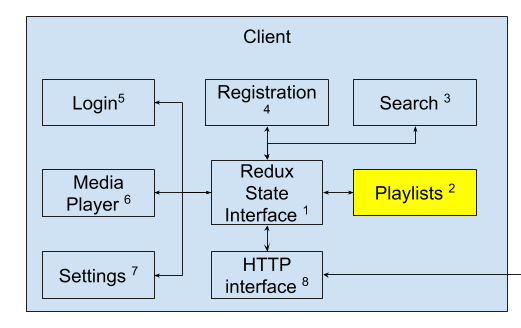
\includegraphics[width=0.60\textwidth]{images/client/client_playlists.png}
 	\caption{Playlist subsystem}
\end{figure}

\subsubsection{Assumptions}
One assumption we have made is that in order to display playlists the user will need to have at least one account connected to Synthify.

\subsubsection{Responsibilities}
The primary responsibility of this subsystem is to provide the user an easy way to view their playlists

\subsubsection{Subsystem Interfaces}
\begin {table}[H]
\caption {Playlist interfaces} 
\begin{center}
    \begin{tabular}{ | p{1cm} | p{6cm} | p{3cm} | p{3cm} |}
    \hline
    ID & Description & Inputs & Outputs \\ \hline
    \#01 & Redux State Interface & \pbox{3cm}{ User Id } & \pbox{3cm}{Playlists for a user}  \\ \hline
    \end{tabular}
\end{center}
\end{table}

\newpage